\documentclass[11pt]{article}
\usepackage[margin=1in]{geometry}
\usepackage{booktabs,amsmath,amssymb,xcolor,graphicx}
\usepackage{tikz}\usetikzlibrary{arrows.meta}
\usepackage{hyperref}\hypersetup{colorlinks=true,linkcolor=blue!50!black,urlcolor=blue!50!black}

\title{\textbf{Splines as KAN activations}\\[2pt]
\large Catmull-Rom, B-spline, Chebyshev, the CR--Chebyshev view, and Kochanek-Bartels}
\author{Aiko (Claude Code), for Dr.\ Csaba Hajdu}\date{2026-06-28 (JST)}

\begin{document}\maketitle

\begin{abstract}
\noindent In HSiKAN every edge carries a \emph{learnable per-channel univariate function} $\varphi_c:\mathbb{R}\to
\mathbb{R}$ --- the KAN activation. Which spline realises $\varphi_c$ sets four things at once: \textbf{expressiveness}
(can it bend sharply?), \textbf{smoothness} (does it regularise?), \textbf{parameter efficiency}, and \textbf{evaluation
cost} (the launch-bound). This note lays out the four bases we use or could use --- Catmull-Rom (the current cell),
cubic B-spline, Chebyshev, and the new \textbf{CR--Chebyshev} hybrid --- plus the Kochanek-Bartels generalisation,
with the maths, rendered curves, and a comparison table.
\end{abstract}

\section{The KAN-activation setting}
A KAN layer replaces fixed scalar activations with learned univariate functions on the edges. Each $\varphi_c$ is
parameterised by a few weights (control points / coefficients) and evaluated on a softly-bounded input
$x\in[-1,1]$. The signed-message-passing of HSiKAN then aggregates $\varphi$-transformed features. So the spline is
the unit of nonlinearity, and its basis is a genuine design axis.

\begin{figure}[h]\centering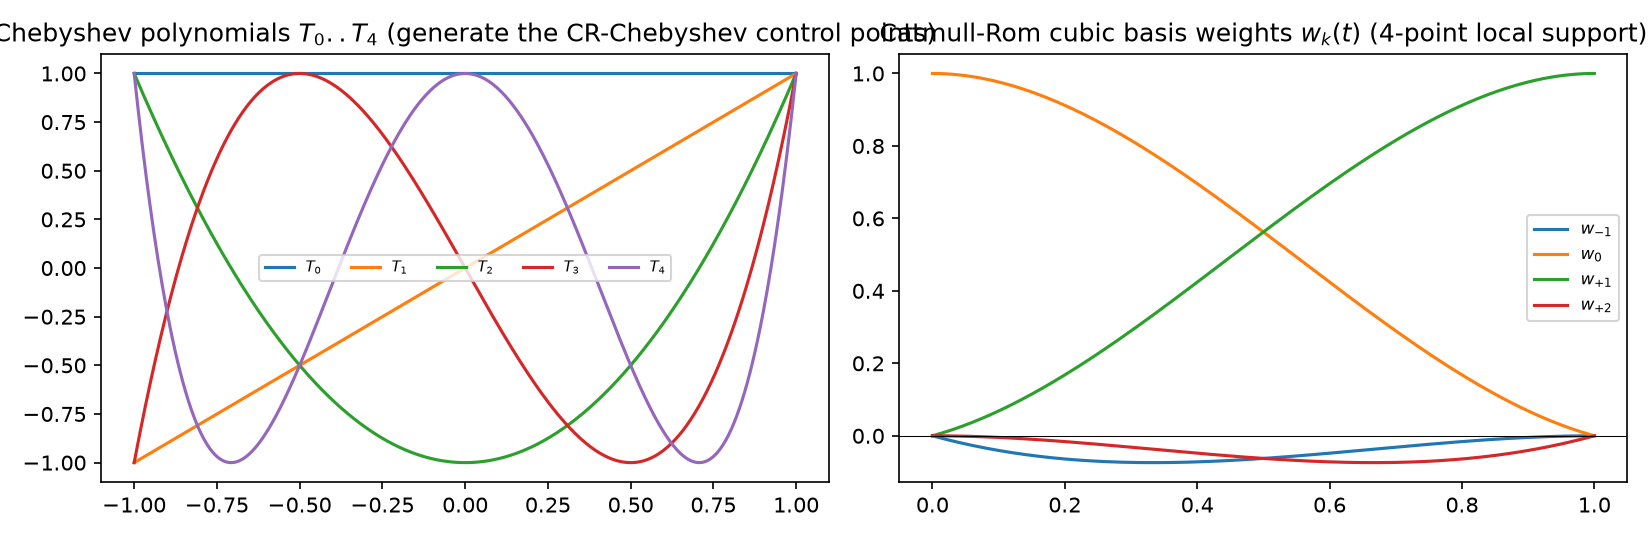
\includegraphics[width=0.96\textwidth]{figures/splines/bases.png}
\caption{Left: the Chebyshev polynomials $T_0..T_4$ (recurrence $T_{n+1}=2xT_n-T_{n-1}$) --- orthogonal on
$[-1,1]$, global support, the generators of the CR--Chebyshev control points. Right: the Catmull-Rom cubic basis
weights $w_k(t)$ --- four-point \emph{local} support, summing to one.}\end{figure}

\section{Catmull-Rom --- interpolating, $C^1$, local (the current cell)}
On the segment between control points $p_i,p_{i+1}$ with $t\in[0,1]$,
\[
P(t)=\!\!\sum_{k=-1}^{2}\! w_k(t)\,p_{i+k},\quad
\begin{aligned}
w_{-1}&=\tfrac12(-t^3+2t^2-t), & w_{0}&=\tfrac12(3t^3-5t^2+2),\\
w_{+1}&=\tfrac12(-3t^3+4t^2+t), & w_{+2}&=\tfrac12(t^3-t^2),
\end{aligned}
\]
equivalently a cubic Hermite with tangents $m_i=\tfrac12(p_{i+1}-p_{i-1})$. It \textbf{interpolates} (the curve
passes through every $p_i$), is $C^1$, has \textbf{local} 4-point support, and can overshoot near sharp data. Cost:
the four control points are \emph{gathered} per sample --- $\sim$45 small ops, the dispatch-bound core of HSiKAN's
forward.

\section{Cubic B-spline --- approximating, $C^2$, smoother}
$P(t)=\sum_i N_{i,3}(t)\,c_i$ with the Cox--de Boor basis $N_{i,k}$ (recursive in the order $k$). Unlike CR, the
curve does \textbf{not} pass through the coefficients $c_i$ --- it \emph{approximates}, staying inside their convex
hull, and is $C^2$ (one degree smoother than CR). The coefficients are control \emph{handles}, not curve values.

\begin{figure}[h]\centering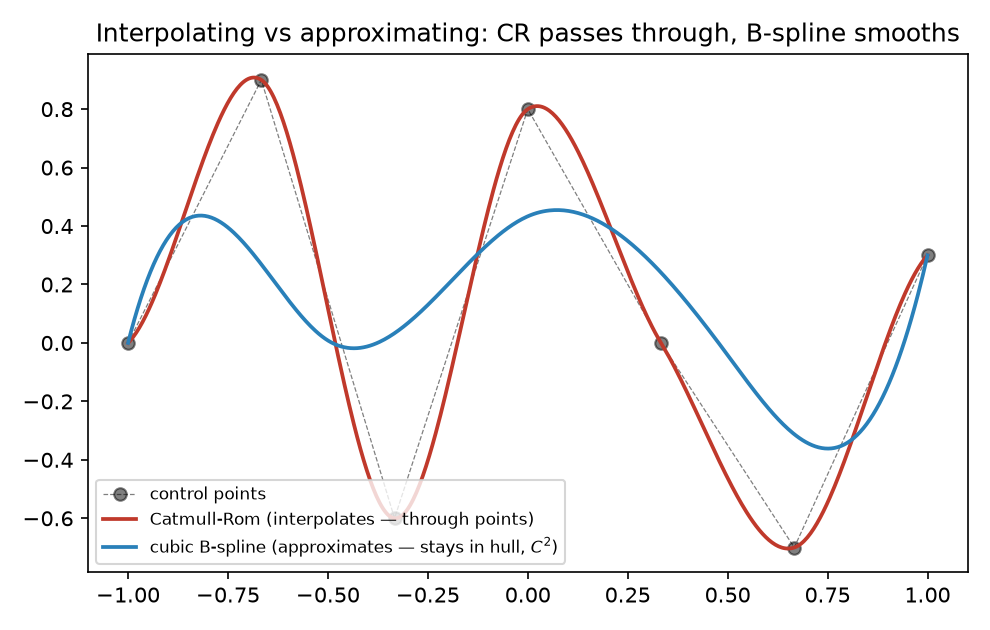
\includegraphics[width=0.62\textwidth]{figures/splines/interp_vs_approx.png}
\caption{Same control points: Catmull-Rom passes through them (interpolating, can overshoot); the cubic B-spline
smooths inside the hull (approximating, $C^2$).}\end{figure}

\section{Chebyshev and the CR--Chebyshev view}
\textbf{Chebyshev:} $T_0{=}1,\,T_1{=}x,\,T_{n+1}{=}2xT_n-T_{n-1}$ --- orthogonal polynomials with the
\emph{minimax} (near-optimal uniform) approximation property, \textbf{global} support, evaluated as a single
Vandermonde \emph{matmul} (no gather, no branching) so they are the cheapest basis at $B{=}1$. A function is written
$f(x)\approx\sum_k c_k T_k(x)$.

\textbf{CR--Chebyshev (the new view):} let the CR control points be \emph{generated} by a degree-$(k{-}1)$
Chebyshev expansion sampled at the fixed knots,
\[
P \;=\; C\,T_{\mathrm{knots}}^{\top},\qquad T_{\mathrm{knots}}\in\mathbb{R}^{G\times k}\ \text{(cached constant)},
\]
with $C\in\mathbb{R}^{(\text{channels})\times k}$ learned. The control points are now a \textbf{band-limited}
(smooth) family rather than free knots --- this is Catmull-Rom seen \emph{through a Chebyshev lens}. Consequences:
$k$ coefficients/channel ($k<G$ $\Rightarrow$ param-efficient), a smoother fit on smooth targets, and --- because
the function lies on a degree-$k$ Chebyshev --- it is Chebyshev-representable, so it can be \textbf{trained with the
CR gather but deployed with the cheap Chebyshev matmul} ($\sim$3$\times$ at $B{=}1$). The honest cost: band-limiting
caps sharp/narrow features; $k$ is the knob.

\begin{figure}[h]\centering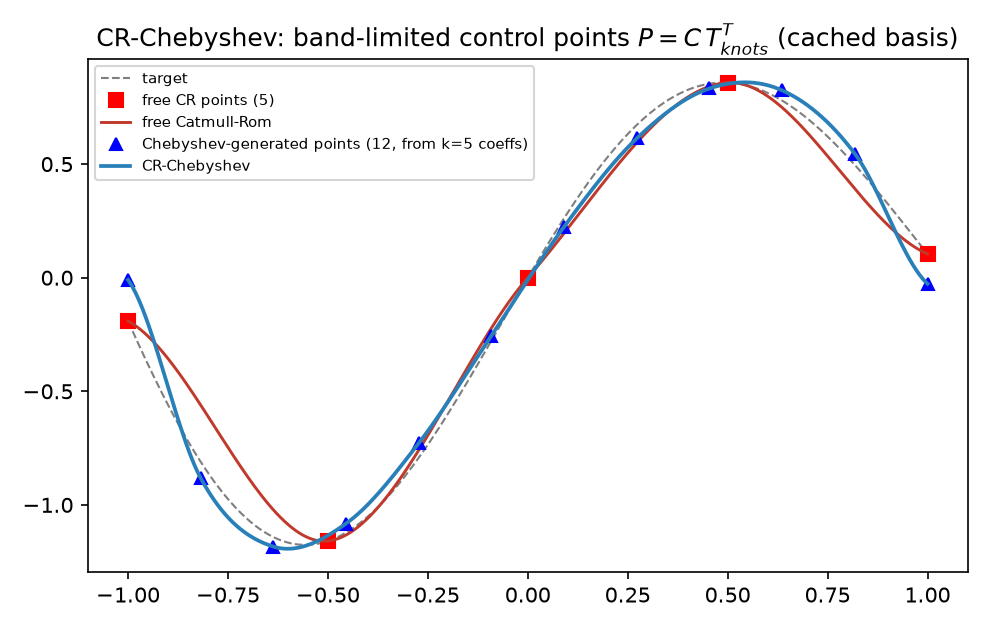
\includegraphics[width=0.62\textwidth]{figures/splines/cr_chebyshev_view.png}
\caption{CR--Chebyshev: $k{=}5$ learned coefficients place $G{=}12$ smooth control points (blue), interpolated by
CR --- closer to the smooth target than 5 free CR points (red), at equal parameter count.}\end{figure}

\section{Kochanek-Bartels --- learnable shape (TCB)}
KB is the cubic-Hermite generalisation whose tangents carry \textbf{Tension, Continuity, Bias}:
\[
m_i^{\text{out}}=\tfrac{(1{-}T)(1{+}B)(1{+}C)}{2}\Delta^-_i+\tfrac{(1{-}T)(1{-}B)(1{-}C)}{2}\Delta^+_i,\quad
m_i^{\text{in}}=\tfrac{(1{-}T)(1{+}B)(1{-}C)}{2}\Delta^-_i+\tfrac{(1{-}T)(1{-}B)(1{+}C)}{2}\Delta^+_i,
\]
with $\Delta^-_i=p_i-p_{i-1}$, $\Delta^+_i=p_{i+1}-p_i$. At $T{=}C{=}B{=}0$ this \emph{is} Catmull-Rom. Made
\textbf{learnable} (per channel, or three global scalars), TCB adds shape degrees of freedom CR cannot express:
tension trades overshoot$\leftrightarrow$taut, continuity sets corner sharpness, bias sets asymmetry. It is
\textbf{orthogonal} to CR--Chebyshev (TCB shapes the \emph{tangents}; Chebyshev shapes the \emph{points}), so the
richest cell is ``Chebyshev points $+$ learnable TCB tangents.''

\begin{figure}[h]\centering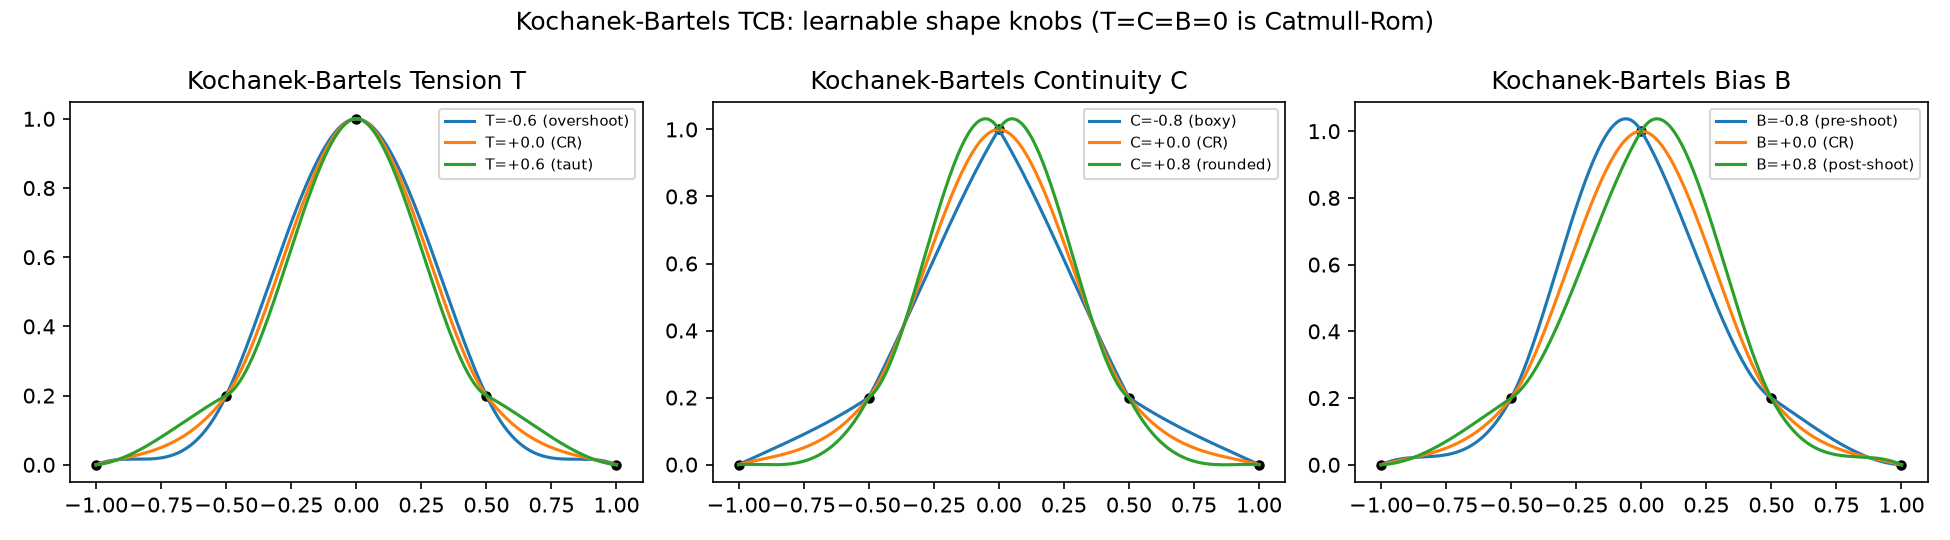
\includegraphics[width=0.98\textwidth]{figures/splines/kb_tcb.png}
\caption{The three Kochanek-Bartels knobs on fixed control points. Tension tightens/overshoots; continuity rounds
or sharpens corners; bias shifts the curve before/after each point. $T{=}C{=}B{=}0$ recovers Catmull-Rom.}\end{figure}

\section{The 3-axis design space --- Catmull-Rom at the origin}
The four constructions are not a list but a \textbf{basis for a design space}: Catmull-Rom sits at the origin and
each generalisation moves along \emph{one} axis.

\begin{center}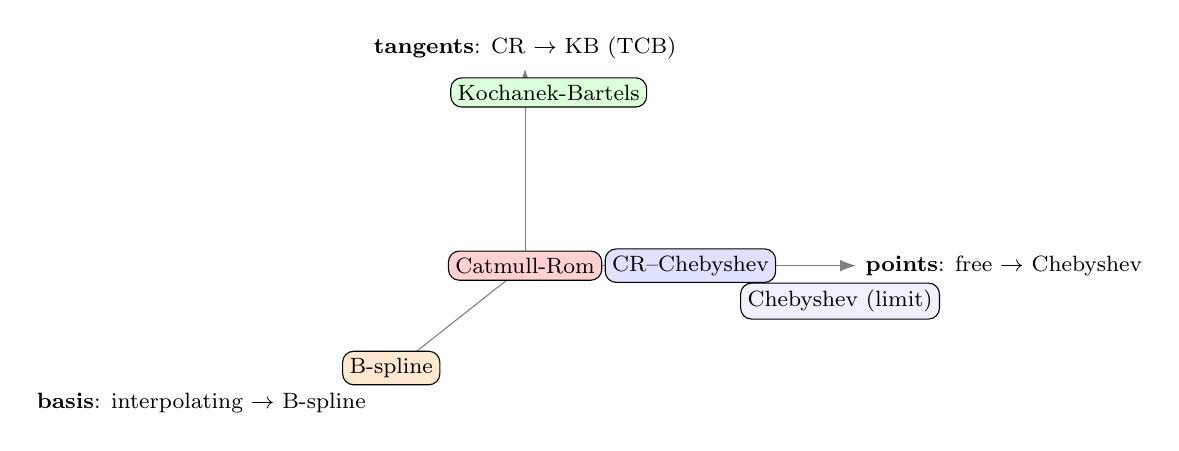
\begin{tikzpicture}[font=\footnotesize,
 c/.style={draw,rounded corners,inner sep=2.5pt},ar/.style={-{Latex[length=2mm]},gray}]
\coordinate (O) at (0,0);
\draw[ar] (O) -- (4.2,0) node[right,black]{\textbf{points}: free $\to$ Chebyshev};
\draw[ar] (O) -- (0,2.5) node[above,black]{\textbf{tangents}: CR $\to$ KB (TCB)};
\draw[ar] (O) -- (-1.9,-1.5) node[below left,black]{\textbf{basis}: interpolating $\to$ B-spline};
\node[c,fill=red!18] at (O) {Catmull-Rom};
\node[c,fill=blue!12] at (2.1,0) {CR--Chebyshev};
\node[c,fill=blue!6] at (4.0,-0.45) {Chebyshev (limit)};
\node[c,fill=green!14] at (0.3,2.2) {Kochanek-Bartels};
\node[c,fill=orange!18] at (-1.7,-1.3) {B-spline};
\end{tikzpicture}\end{center}

\textbf{Axis 1 --- control points (a smoothness prior on the knots):} free points $\to$ band-limited Chebyshev
expansion. More Chebyshev = fewer parameters, smoother, cheaper, but a lower fit ceiling; the \emph{pure}
Chebyshev (no gather) is the global limit. \textbf{Axis 2 --- tangents:} fixed Catmull-Rom $\to$ learnable
Kochanek-Bartels TCB --- the same fit on these targets but extra shape degrees of freedom (overshoot, corners,
bias). \textbf{Axis 3 --- basis mode:} interpolating Hermite (CR/KB pass through the points) $\to$ approximating
B-spline ($C^2$, stays in the hull). They \textbf{compose} (e.g.\ Chebyshev points $+$ TCB tangents); axes 1--2
are orthogonal \emph{within} the interpolating family, while axis 3 switches the basis itself (a B-spline has no
explicit tangents, so it does not carry axis 2). \textbf{So B-splines are not omitted --- they are the third
axis.}

\begin{table}[h]\centering\small
\begin{tabular}{lcccccc}
\toprule
basis & smooth & bump & sharp & $B{=}1\,\mu s$ & $B{=}256\,\mu s$ & params \\
\midrule
Catmull-Rom (origin) & 0.0001 & 0.0004 & 0.0000 & 656 & 802 & 8 \\
B-spline (axis 3) & 0.0000 & 0.0001 & 0.0001 & 757 & 1236 & 10 \\
Chebyshev (axis 1 limit) & 0.0004 & 0.0004 & 0.0022 & \textbf{319} & \textbf{389} & 8 \\
CR--Chebyshev (axis 1) & 0.0039 & 0.0104 & 0.0350 & 442 & 476 & \textbf{5} \\
Kochanek-Bartels (axis 2) & 0.0001 & 0.0003 & 0.0000 & 754 & 741 & 11 \\
\bottomrule
\end{tabular}
\caption{Measured: gradient-fit MSE to each target (1 channel, 400 Adam steps) $+$ latency $+$ params. CR / B-spline
/ KB have the degrees of freedom to fit anything; pure Chebyshev is the fastest but band-limits the \emph{sharp}
target; CR--Chebyshev is the param-efficient, smooth, fast \emph{middle} --- fewest params, a built-in smoothness
\emph{regulariser} --- at a deliberately lower fit ceiling; B-spline is $C^2$-smooth but slowest batched. The cell
choice is therefore a point in the cube, picked by what a layer needs: raw local fit (CR), speed (Chebyshev),
parameter-efficiency/regularisation (CR--Chebyshev), shape control (KB), or $C^2$ smoothness (B-spline).}
\end{table}

\section{Which, for HSiKAN}
\textbf{CR--Chebyshev} is the new default cell for SA-HSiKAN (shipped, tested): smoother and param-efficient, with
the train-CR / deploy-Chebyshev bridge that helps the launch-bound rollout. \textbf{Kochanek-Bartels} is the
expressiveness ablation when a channel needs sharp or asymmetric shape. \textbf{Chebyshev-only} is the fast
deploy form. Plain \textbf{Catmull-Rom} stays the interpolation baseline. All are one \texttt{make\_activation}
call apart (\texttt{cr} / \texttt{cr\_cheby} / \texttt{bspline}), so the choice is a config, not a fork.
\end{document}
